\documentclass[10pt,a4paper]{article}
\usepackage[T1]{fontenc}
\usepackage[utf8]{inputenc}
\usepackage{lmodern}
\usepackage[margin=0.82in]{geometry}
\usepackage{amsmath,amssymb,amsthm,mathtools}
\usepackage{graphicx}
\usepackage{microtype}
\usepackage{xcolor}
\usepackage[colorlinks=true,linkcolor=blue!50!black,citecolor=blue!50!black,urlcolor=blue!50!black]{hyperref}

\newtheorem{theorem}{Theorem}
\newtheorem{proposition}[theorem]{Proposition}
\newtheorem{lemma}[theorem]{Lemma}
\newtheorem{corollary}[theorem]{Corollary}

\newcommand{\ket}[1]{\lvert #1\rangle}
\newcommand{\bra}[1]{\langle #1\rvert}
\newcommand{\ketbra}[2]{\lvert #1\rangle\langle #2\rvert}
\newcommand{\id}{\mathbf{1}}
\newcommand{\tr}{\operatorname{Tr}}
\newcommand{\G}{\Gamma}
\newcommand{\uW}{u_W}
\newcommand{\lmax}{\lambda_{\max}}
% ---- AI disclosure statement (IOP Publishing asks for one when AI contributed to the preparation):
% ---- shown by default; set \showackfalse only if the statement is supplied to the journal elsewhere.
\newif\ifshowack \showackfalse
\setlength{\parskip}{1pt plus 1pt}
\makeatletter
\renewcommand\section{\@startsection{section}{1}{\z@}{-1.6ex plus -.6ex}{0.7ex}{\normalfont\large\bfseries}}
\makeatother

\hypersetup{pdftitle={Comment on "Mirrored entanglement witnesses for multipartite and high-dimensional quantum systems"},
  pdfauthor={Ruqing Chen}}

\title{\vspace{-1.6cm}\Large Comment on ``Mirrored entanglement witnesses for multipartite and
high-dimensional quantum systems'' (Quantum Sci.\ Technol.\ 11, 015037 (2026))}
\author{Ruqing Chen\\[1pt]
\small GUT Geoservice Inc., Montreal, Quebec, Canada\\
\small \href{mailto:ruqing@hotmail.com}{ruqing@hotmail.com}\quad
ORCID: \href{https://orcid.org/0009-0009-4622-6615}{0009-0009-4622-6615}}
\date{\small November 27, 2026}

\begin{document}
\maketitle
\vspace{-0.9cm}
\begin{abstract}\noindent
In Section~4.2.1 of the article by Seong \emph{et al}~\cite{SBHCB26}, the mirrored
operator of the $4\otimes4$ entanglement witness $W[1,1,1,0]$ is given as
$\tfrac43\id-W[1,1,1,0]$ and is stated to be a non-decomposable witness, from which it is
concluded that two non-decomposable witnesses can be mirrored with each other. This
operator has the expectation value $-1/6$ on a product state and is not an entanglement
witness. The correct separable bound is $3/2$, and the corrected mirror is decomposable.
We determine the separable bound exactly for the whole circulant covariant family of
Proposition~5 of~\cite{SBHCB26} in every dimension and show that no operator of this
family has a non-decomposable mirror, which bears on the first open problem
of~\cite{SBHCB26}. Non-decomposable mirrored pairs do exist in every $n\otimes n$,
$n\ge4$, outside the family. We also locate two slips in Appendix~C.4
of~\cite{SBHCB26} that affect its three-qubit example, and list some smaller corrections.
\end{abstract}

\section{The \texorpdfstring{$4\otimes4$}{4x4} example of Section~4.2.1}\label{sec:counter}

All section, page and equation numbers of~\cite{SBHCB26} refer to the published article.
Let $n\ge2$, let $\ket{i,j}$ be the product basis of $\mathbb{C}^n\otimes\mathbb{C}^n$
with indices modulo $n$, and for real $\alpha=(\alpha_0,\dots,\alpha_{n-1})$ let
\begin{equation}\label{eq:Walpha}
W_\alpha=\sum_{i,k}\alpha_k\ketbra{i,i+k}{i,i+k}-\sum_{i\neq j}\ketbra{ii}{jj}.
\end{equation}
These are the operators of Proposition~5 of~\cite{SBHCB26} (Eq.~(68), p.~24), here with
arbitrary real coefficients; for $n=4$ they are the operators $W[a,b,c,d]$ of Eq.~(72)
with $\alpha=(a,b,c,d)$. Recall~\cite{BCH20} that the mirrored operator of a witness $W$ is
$M=\uW\id-W$, where $\uW=\max_{\ket{e},\ket{f}}\bra{e,f}W\ket{e,f}$ is the separable upper
bound; $\mu\id-W$ is non-negative on separable states if and only if $\mu\ge\uW$.

\begin{lemma}\label{lem:prod}
For unit vectors $e,f\in\mathbb{C}^n$ let $s_k=\sum_i|e_i|^2|f_{i+k}|^2$. Then
$\sum_ks_k=1$ and
$\bra{e,f}W_\alpha\ket{e,f}=\sum_{k}\alpha_ks_k+s_0-\bigl|\sum_ie_if_i\bigr|^{2}$.
\end{lemma}
\begin{proof}
The diagonal part gives $\sum_k\alpha_ks_k$, and
$\sum_{i\neq j}\overline{e_if_i}\,e_jf_j=|\sum_ie_if_i|^2-s_0$.
\end{proof}

On p.~25 of~\cite{SBHCB26} the mirrored operator of $W(0)=W[1,1,1,0]$ is stated to be
$M[1,1,1,0]=\tfrac43\,\id_4\otimes\id_4-W[1,1,1,0]$. Take
\begin{equation}\label{eq:psistar}
\ket{e}=\tfrac{1}{\sqrt2}(\ket0+\ket2),\qquad\ket{f}=\tfrac{1}{\sqrt2}(\ket0-\ket2).
\end{equation}
Then $s_0=s_2=\tfrac12$, $s_1=s_3=0$ and $\sum_ie_if_i=0$, so by Lemma~\ref{lem:prod}
\begin{equation}\label{eq:threehalves}
\bra{e,f}W[1,1,1,0]\ket{e,f}=\tfrac12+\tfrac12+\tfrac12=\tfrac32>\tfrac43,\qquad
\bra{e,f}\bigl(\tfrac43\id-W[1,1,1,0]\bigr)\ket{e,f}=-\tfrac16 .
\end{equation}
The operator $M[1,1,1,0]$ of~\cite{SBHCB26} is negative on a product state and is
therefore not an entanglement witness (Fig.~\ref{fig:one}(a)). The statements that follow
from it on p.~25, ``the mirrored operator $M[1,1,1,0]$ is a non-decomposable EW. We have
shown that a pair of non-decomposable EWs can be mirrored with each other'', and the
corresponding sentence of Section~1.5 (p.~6), are not established. The value $4/3$ is
the separable bound of the three-dimensional Choi witness $W[1,1,0]$; it is not the bound
in dimension four.

\section{Exact separable bound and decomposability in all dimensions}\label{sec:exact}

An operator is decomposable if it equals $P+Q^{\G}$ with $P,Q\ge0$, where $\G$ is the
partial transpose on the first factor. Decomposable operators are non-negative on all PPT
states. Let $\ket{\phi^+}=n^{-1/2}\sum_i\ket{ii}$. The spectrum of $W_\alpha$ gives
$\lmax(W_\alpha)=\max\{\alpha_0+1,\alpha_1,\dots,\alpha_{n-1}\}$.

\begin{theorem}[Decomposition certificate]\label{thm:cert}
Let $v\in\mathbb{R}$ and $\lambda\in[0,1]$ satisfy
$v\ge\alpha_0+\lambda$, $v\ge\alpha_k$ and
$(v-\alpha_k)(v-\alpha_{n-k})\ge(1-\lambda)^{2}$ for $1\le k\le n-1$.
Then $v\,\id-W_\alpha=P+Q^{\G}$ with the positive semidefinite operators
\begin{equation}\label{eq:PQ}
P=n\lambda\,\ketbra{\phi^+}{\phi^+}+(v-\alpha_0-\lambda)\sum_i\ketbra{ii}{ii},\qquad
Q=\sum_i\sum_{k=1}^{n-1}(v-\alpha_k)\ketbra{i,i+k}{i,i+k}
+(1-\lambda)\sum_{i\neq j}\ketbra{i,j}{j,i}.
\end{equation}
\end{theorem}
\begin{proof}
$P\ge0$ is evident. $Q$ vanishes on the vectors $\ket{ii}$ and is block diagonal on the
pairs $\{\ket{i,j},\ket{j,i}\}$, $i\neq j$, with the $2\times2$ blocks that have the
diagonal entries $v-\alpha_k$, $v-\alpha_{n-k}$ ($k=j-i$) and the off-diagonal entry
$1-\lambda$; these are positive semidefinite by assumption. Partial transposition fixes
the diagonal of $Q$ and maps $\ketbra{i,j}{j,i}$ to $\ketbra{j,j}{i,i}$. Thus $P+Q^{\G}$
has the entries $\lambda+(1-\lambda)=1$ on $\ketbra{ii}{jj}$, $i\neq j$, the entries
$v-\alpha_0$ on $\ket{ii}$ and $v-\alpha_k$ on $\ket{i,i+k}$, which are those of
$v\,\id-W_\alpha$.
\end{proof}

For $1\le k\le n/2$ let
$B_k(\alpha)=\bigl((\alpha_0+1)^{2}-\alpha_k\alpha_{n-k}\bigr)/\bigl(2(\alpha_0+1)-\alpha_k-\alpha_{n-k}\bigr)$
if $\alpha_0+1>\max(\alpha_k,\alpha_{n-k})$, and $B_k(\alpha)=-\infty$ otherwise.

\begin{theorem}[Exact separable bound]\label{thm:exact}
For all $n\ge2$ and all $\alpha\in\mathbb{R}^n$,
\begin{equation}\label{eq:L}
\uW=L_n(\alpha):=\max\bigl\{\alpha_0,\alpha_1,\dots,\alpha_{n-1},\,
B_1(\alpha),\dots,B_{\lfloor n/2\rfloor}(\alpha)\bigr\},
\end{equation}
the maximum is attained on a product vector supported on at most two levels, and
$L_n(\alpha)\,\id-W_\alpha$ is decomposable.
\end{theorem}
\begin{proof}
\emph{Lower bound.} The basis vector $\ket{i,i+k}$ gives $\alpha_k$. The vector
$(\sqrt t\,\ket i+\sqrt{1-t}\,\ket{i+k})\otimes(\sqrt{1-t}\,\ket i-\sqrt t\,\ket{i+k})$
has $\sum_ie_if_i=0$ and, by Lemma~\ref{lem:prod}, the value
$g_k(t)=2(\alpha_0+1)t(1-t)+\alpha_kt^{2}+\alpha_{n-k}(1-t)^{2}$. If
$\alpha_0+1>\max(\alpha_k,\alpha_{n-k})$, this quadratic is strictly concave with maximum
$B_k(\alpha)$ at
$t^{*}=(\alpha_0+1-\alpha_{n-k})/(2(\alpha_0+1)-\alpha_k-\alpha_{n-k})\in(0,1)$.
\emph{Upper bound.} Put $L=L_n(\alpha)$ and apply Theorem~\ref{thm:cert} with $v=L$ and
$\lambda=\min(1,L-\alpha_0)\in[0,1]$. The first two conditions hold by the definition of
$L$. If $\lambda=1$ the third is $(L-\alpha_k)(L-\alpha_{n-k})\ge0$. If
$\lambda=L-\alpha_0<1$, then $\alpha_0+1>L\ge\max(\alpha_k,\alpha_{n-k})$ and the third
condition, $(\alpha_0+1-L)^2\le(L-\alpha_k)(L-\alpha_{n-k})$, is equivalent to
$L\ge B_k(\alpha)$. Hence $L\,\id-W_\alpha$ is decomposable, so block positive, and
$\uW\le L$.
\end{proof}

\begin{corollary}[No non-decomposable mirror]\label{cor:nogo}
For every $n\ge2$, $\alpha\in\mathbb{R}^n$ and $\mu\in\mathbb{R}$, the operator
$\mu\id-W_\alpha$ is block positive if and only if $\mu\ge L_n(\alpha)$, if and only if it
is decomposable. It is not block positive for $\mu<L_n(\alpha)$, a decomposable witness
for $L_n(\alpha)\le\mu<\lmax(W_\alpha)$, and positive semidefinite for
$\mu\ge\lmax(W_\alpha)$. In no dimension is it a non-decomposable witness.
\end{corollary}
\begin{proof}
For $\mu\ge L_n(\alpha)$, $\mu\id-W_\alpha=(\mu-L_n)\id+(L_n\id-W_\alpha)$ is the sum of a
positive and a decomposable operator. The rest follows from Theorem~\ref{thm:exact}.
\end{proof}

\begin{figure}[t]
\centering
\begin{minipage}[c]{0.275\textwidth}\centering
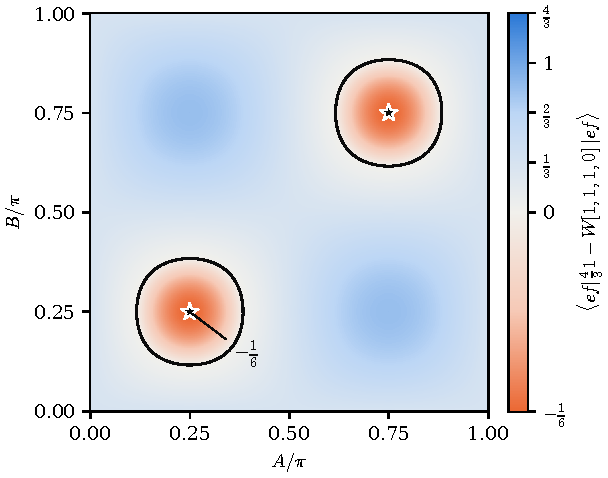
\includegraphics[width=\textwidth]{fig_negative_region.pdf}\\[-2pt]{\small (a)}
\end{minipage}\hfill
\begin{minipage}[c]{0.715\textwidth}\centering
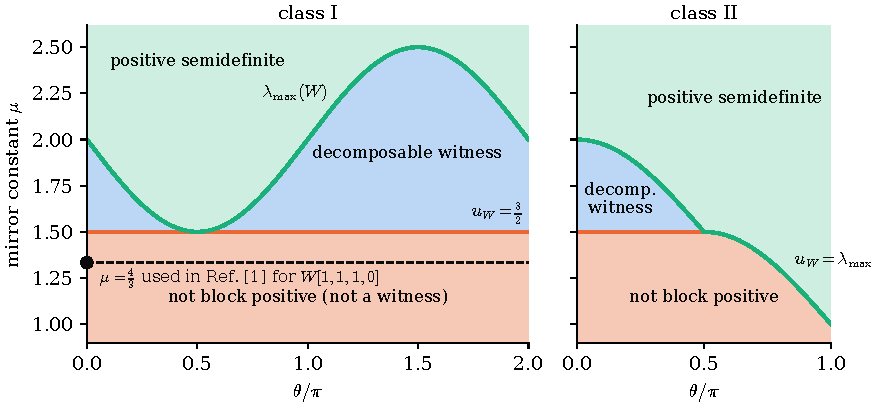
\includegraphics[width=\textwidth]{fig_phase_diagram.pdf}\\[-2pt]{\small (b)}
\end{minipage}
\caption{(a) Expectation value of $\tfrac43\id-W[1,1,1,0]$ on the product vectors
$\ket e=\cos A\ket0+\sin A\ket2$, $\ket f=\cos B\ket0-\sin B\ket2$; inside the black
curves it is negative, with minimum $-1/6$ at the vector \eqref{eq:psistar} (stars).
(b) Nature of $\mu\id-W$ for classes I and II of~\cite{SBHCB26} as a function of the
mirror constant $\mu$: not block positive below $\uW$, a decomposable witness between
$\uW$ and $\lmax(W)$, positive semidefinite above. There is no region of non-decomposable
mirrors. The dot marks the operator $M[1,1,1,0]$ of~\cite{SBHCB26}.}
\label{fig:one}
\end{figure}

\emph{Dimension four.} For $W[a,b,c,d]$, Eq.~\eqref{eq:L} reads
$\uW=\max\{a,b,c,d,\tfrac12(a+c+1),B_1\}$ with
$B_1=((a+1)^2-bd)/(2(a+1)-b-d)$ if $a+1>\max(b,d)$. For $W[1,\dots,1,0]$ in dimension
$n$ one has $B_1=4/3$, and $B_k=3/2$ for $2\le k\le n/2$: the bound is $4/3$ for $n=3$
and $3/2$ for every $n\ge4$, because product vectors on two non-neighbouring levels first
exist for $n=4$. For $W[1,1,1,0]$, Theorem~\ref{thm:cert} with $v=\tfrac32$,
$\lambda=\tfrac12$ gives the identity, which can be checked by hand,
\begin{equation}\label{eq:dec1110}
\begin{aligned}
\tfrac32\id-W[1,1,1,0]&=2\ketbra{\phi^+}{\phi^+}+Q_0^{\,\G},\\
Q_0&=\sum_i\Bigl[\tfrac12\ketbra{i,i+1}{i,i+1}+\tfrac12\ketbra{i,i+2}{i,i+2}
+\tfrac32\ketbra{i,i+3}{i,i+3}\Bigr]+\tfrac12\sum_{i\neq j}\ketbra{i,j}{j,i},
\end{aligned}
\end{equation}
where $Q_0\ge0$ has the eigenvalues $0$, $1-\tfrac1{\sqrt2}$, $1$, $1+\tfrac1{\sqrt2}$.
Together with \eqref{eq:threehalves} this shows that the mirrored operator of
$W[1,1,1,0]$ is $\tfrac32\id-W[1,1,1,0]$ and that it is decomposable. For the PPT states
$\rho_x$ of Eq.~(75) of~\cite{SBHCB26} we confirm the printed value
$\tr[(\tfrac43\id-W[1,1,1,0])\rho_x]=4(x^2-5x+4)/(3x)$, but with the correct constant
\begin{equation}\label{eq:rhox}
\tr\bigl[(\tfrac32\id-W[1,1,1,0])\rho_x\bigr]=\frac{2\bigl((x-1)^{2}+2\bigr)}{x}>0
\qquad(x>0),
\end{equation}
so the states $\rho_x$ are not detected. The same holds for both classes
of~\cite{SBHCB26}. For class~I (Eq.~(74), where $d=\mu-b$ is to be read as $d=1-b$),
$\uW=\tfrac12(a+c+1)=\tfrac32$ for every $\theta$, attained on \eqref{eq:psistar}, and
Theorem~\ref{thm:cert} with $v=\tfrac32$, $\lambda=\tfrac12(1+\sin\theta)$ gives
$\tfrac32\id-W_{\mathrm I}(\theta)=2(1+\sin\theta)\ketbra{\phi^+}{\phi^+}+Q_\theta^{\,\G}$;
the required inequality is
$(\tfrac32-b)(\tfrac32-d)=\tfrac14(3+\sin^2\theta)\ge\tfrac14(1-\sin\theta)^2$. For
class~II (Eq.~(76)), $\uW=B_1=\tfrac32$ for $\theta\in[0,\pi/2]$ and
$\uW=d=\lmax(W)$ for $\theta\in[\pi/2,\pi]$, in agreement with the statement
of~\cite{SBHCB26} that these mirrors are decomposable witnesses or positive semidefinite.
Fig.~\ref{fig:one}(b) shows both classes.

\emph{Open problem~1 of~\cite{SBHCB26}.} Section~6 (item~1, p.~29) asks whether mirrored
pairs of optimal witnesses exist in higher dimensions and suggests to seek them among
covariant Bell-diagonal witnesses. The operators \eqref{eq:Walpha} are covariant and Bell
diagonal. By Corollary~\ref{cor:nogo}, in no dimension does this family contain a mirrored
pair in which both members detect PPT entangled states, and so it contains no analogue of
the $3\otimes3$ pair of~\cite{CBBH25}. The corollary needs no optimality assumption; it
does not exclude a pair of optimal witnesses one of which is decomposable, and it does not
cover covariant operators that are not circulant (Eq.~(67) of~\cite{SBHCB26}).

\section{Higher-dimensional pairs, Appendix~C.4, and further corrections}\label{sec:further}

\begin{proposition}[Embedding]\label{prop:embed}
Let $W_3,M_3$ be non-decomposable witnesses on $\mathbb{C}^3\otimes\mathbb{C}^3$ with
$W_3+M_3=\mu\,\id$. For $n\ge4$ let $V:\mathbb{C}^3\to\mathbb{C}^n$ be the inclusion of
the first three basis vectors and $\Pi=VV^{\dagger}\otimes VV^{\dagger}$. Then
$W_n=(V\otimes V)W_3(V\otimes V)^{\dagger}+\tfrac{\mu}{2}(\id-\Pi)$ and
$M_n=(V\otimes V)M_3(V\otimes V)^{\dagger}+\tfrac{\mu}{2}(\id-\Pi)$ are non-decomposable
witnesses on $\mathbb{C}^n\otimes\mathbb{C}^n$ with $W_n+M_n=\mu\,\id$.
\end{proposition}
\begin{proof}
$\mu\ge0$, as $\mu=\bra{e,f}(W_3+M_3)\ket{e,f}$. With $e'=V^{\dagger}e$,
$f'=V^{\dagger}f$ one has
$\bra{e,f}W_n\ket{e,f}=\bra{e',f'}W_3\ket{e',f'}+\tfrac\mu2(1-\|e'\|^2\|f'\|^2)\ge0$. If
$\rho$ is a PPT state with $\tr(W_3\rho)<0$, then $(V\otimes V)\rho(V\otimes V)^{\dagger}$
is a PPT state, because $V$ is a real isometry, and has the same negative expectation
value with $W_n$. The same holds for $M_n$.
\end{proof}

Applied to the optimal pair of Eq.~(77) of~\cite{SBHCB26}, which is due
to~\cite{CBBH25} and for which we confirm $W+M=4\,\id$ and
$\tr(W\rho_W)=\tr(M\rho_M)=-\tfrac25$, this gives a mirrored pair of non-decomposable
witnesses in every $n\otimes n$, $n\ge4$. The sentence of~\cite{SBHCB26} quoted in
Section~\ref{sec:counter} is therefore true as an existence statement, although not for
the example given there and not within the family \eqref{eq:Walpha}. We make no claim
about optimality of $W_n$ and $M_n$.

\emph{Appendix~C.4 and the three-qubit state $\rho(b,c)$.} For the witnesses
$W[i_1,i_2,i_3]$ of Eq.~(60) and the state $\rho(b,c)$ of Eq.~(64) (p.~22),
Section~3.3.2 and Table~2 of~\cite{SBHCB26} state
$\tr[W[1,1,0]\rho(b,c)]=2(c-3)/(b+c+6)$. The printed operator and state give instead
\begin{equation}\label{eq:rbc}
\tr\bigl[W[1,1,0]\,\rho(b,c)\bigr]=\frac{2(c+7)}{b+c+6}>0 .
\end{equation}
The derivation in Appendix~C.4 contains two slips. Since
$Y\otimes Y\ket{00}=-\ket{11}$, every Pauli string with two factors $Y$ has the matrix
element $-1$ between $\ket{000}$ and $\ket{111}$, and for the X-shaped state
$\rho_{\mathrm{ppt}}$ with coherences $u_1,\dots,u_4$
\begin{equation}\label{eq:rexact}
r_{122}=\tfrac{2}{\nu}\Re(-u_1+u_2+u_3-u_4),\quad
r_{212}=\tfrac{2}{\nu}\Re(-u_1+u_2-u_3+u_4),\quad
r_{221}=\tfrac{2}{\nu}\Re(-u_1-u_2+u_3+u_4).
\end{equation}
(i)~On p.~36, $r_{122}$ is printed correctly, but $r_{212}$ and $r_{221}$ are printed
with the opposite overall sign. (ii)~On p.~37, for $u_1=u_2=u_4=-1$, $u_3=1$, the
coefficient $r_{122}$ is given as $0$, whereas the expression of p.~36 gives
$\tfrac2\nu(1-1+1+1)=4/(b+c+6)$. The correct values are
$(r_{122},r_{212},r_{221})=(4,-4,4)/(b+c+6)$ in place of the printed $(0,4,-4)/(b+c+6)$;
$r_{333}$ and $r_{111}$ are correct. With Eq.~(139) of~\cite{SBHCB26} this gives
\eqref{eq:rbc}. An independent check uses Appendix~C.3 of~\cite{SBHCB26}, which is
correct: by Eqs.~(131), (133) and (134), $W[1,1,0]$ has the anti-diagonal entry $4$ on the
pair $\{\ket{010},\ket{101}\}$ only and the diagonal entries $2$ on
$\ket{001},\ket{010},\ket{100},\ket{111}$, so that
$(b+c+6)\tr[W[1,1,0]\rho(b,c)]=2(3+c)+8u_3=2c+14$. For the eight witnesses of Eq.~(60) the
expectation value is $2(c+7)/(b+c+6)$ for the labels $[0,0,0]$, $[0,1,0]$, $[0,1,1]$,
$[1,1,0]$ and $2(c-1)/(b+c+6)$ for $[0,0,1]$, $[1,0,0]$, $[1,0,1]$, $[1,1,1]$. The state
$\rho(b,c)$ is therefore detected by, e.g., $W[1,0,0]$ for $0<c<1$, not by $W[1,1,0]$ for
$0<c<3$; the corresponding entry of Table~2 changes from $|c-3|$ to $|c-1|$. The
conclusion of Section~3.3.2 that an optimal mirrored pair detects these PPT states is not
affected.

\emph{Further corrections.} They do not affect the conclusions of~\cite{SBHCB26}.
(1)~Section~5, p.~28: $\tr[W\rho_x]=a+bx+c+d/x-3$ does not hold for the state $\rho_x$ of
Eq.~(75), for which the value is $3a+bx+c+d/x+3>0$; it holds for the PPT state with
diagonal weights $(1,x,1,1/x)$ and entries $+1$ on $\ketbra{ii}{jj}$.
(2)~Section~3.3.2, p.~22, and Table~2: the value $2(x+y+z^{-1}-3)/\nu$ is
$\tr[W[0,1,1]\rho(x,y,z)]$; for the label $W[0,1,0]$ used there, Eq.~(60) gives
$2(x+y+z^{-1}+1)/\nu>0$.
(3)~Section~3.1.1, p.~14: the printed pairs $(W_c,M_c)$ and $(W_{2m},M_{2m})$ do not sum
to a multiple of the identity; one has
$\mu_c\id-W_c=\ketbra{GHZ_n}{GHZ_n}/(2^{n-1}-1)$ and
$(2^n-2)W_{2m}+(2^n+2)M_{2m}=2\,\id$.
(4)~Below Eq.~(40), p.~14: $\id\otimes Y\otimes\id\otimes Y\otimes\cdots$ maps $W_a$ to
$M_a$ only if the number $\lfloor n/2\rfloor$ of factors $Y$ is odd; it fails for
$n=4,5$ ($Z\otimes Y\otimes\id\otimes Y$ works for $n=4$).
(5)~Eqs.~(49), (50) and Table~1, p.~16: $\|W_a\|_{\mathrm{op}}=(2n-1)/((n-1)2^n)$, not
$n/((n-1)2^n)$, so that Eq.~(8) gives the tolerance $1/(2(2n-1))$, not $1/(2n)$; Section~3.2
(p.~17) and Table~2 give $1/(2n-1)$ for the same witness up to a positive factor.
(6)~In several places the symbol $\mu$ is printed where the numeral $1$ is meant, e.g.\
$\mathbb{J}_{k\ell}=\mu$ below Eq.~(69), $d=\mu-b$ in Eq.~(74), and $u_3=\mu$,
$s_1=s_2=s_3=\mu$ on p.~37.

\paragraph{Data and code availability.} All statements above are proved in the text or
can be checked by hand. A script that reproduces them in exact rational or symbolic
arithmetic, including Theorems~\ref{thm:cert} and~\ref{thm:exact} for $n=2,\dots,8$, is
available at \url{https://github.com/Ruqing1963/circulant-covariant-witness-bounds}.

\ifshowack
\paragraph{AI disclosure statement.} Generative AI tools (Claude, Anthropic; Gemini, Google) were
used under the author's direction in drafting and typesetting the text, in cross-checking
algebra, and in writing the verification script. The author has checked all proofs and
computations and is solely responsible for the content.
\fi

\begin{thebibliography}{9}\small\setlength{\itemsep}{0pt}
\bibitem{SBHCB26} J.~Seong, A.~Bera, B.~C.~Hiesmayr, D.~Chru\'sci\'nski, and J.~Bae,
Mirrored entanglement witnesses for multipartite and high-dimensional quantum systems,
Quantum Sci.\ Technol.\ \textbf{11}, 015037 (2026), doi:10.1088/2058-9565/ae30a3.
\bibitem{BCH20} J.~Bae, D.~Chru\'sci\'nski, and B.~C.~Hiesmayr,
Mirrored entanglement witnesses, npj Quantum Inf.\ \textbf{6}, 15 (2020).
\bibitem{CBBH25} D.~Chru\'sci\'nski, A.~Bera, J.~Bae, and B.~C.~Hiesmayr,
A mirrored pair of optimal non-decomposable entanglement witnesses for two qudits does
exist, Sci.\ Rep.\ \textbf{15}, 28205 (2025).
\end{thebibliography}
\end{document}
